\chapter{Ancillary Representation Analyses Figures}

\section{RNN Architecture Learned Representations}
\label{rnn_architecture_representations}

\section{MLP Architecture Learned Representations}
\label{mlp_architecture_representations}

\section{RNN Architecture with environmental and game events covariates learned representations}
\label{rnn_env_even_architecture_representations}

\section{Partitions behavioural metrics representations}
\label{partitions_behavioural}

\begin{figure}[ht]
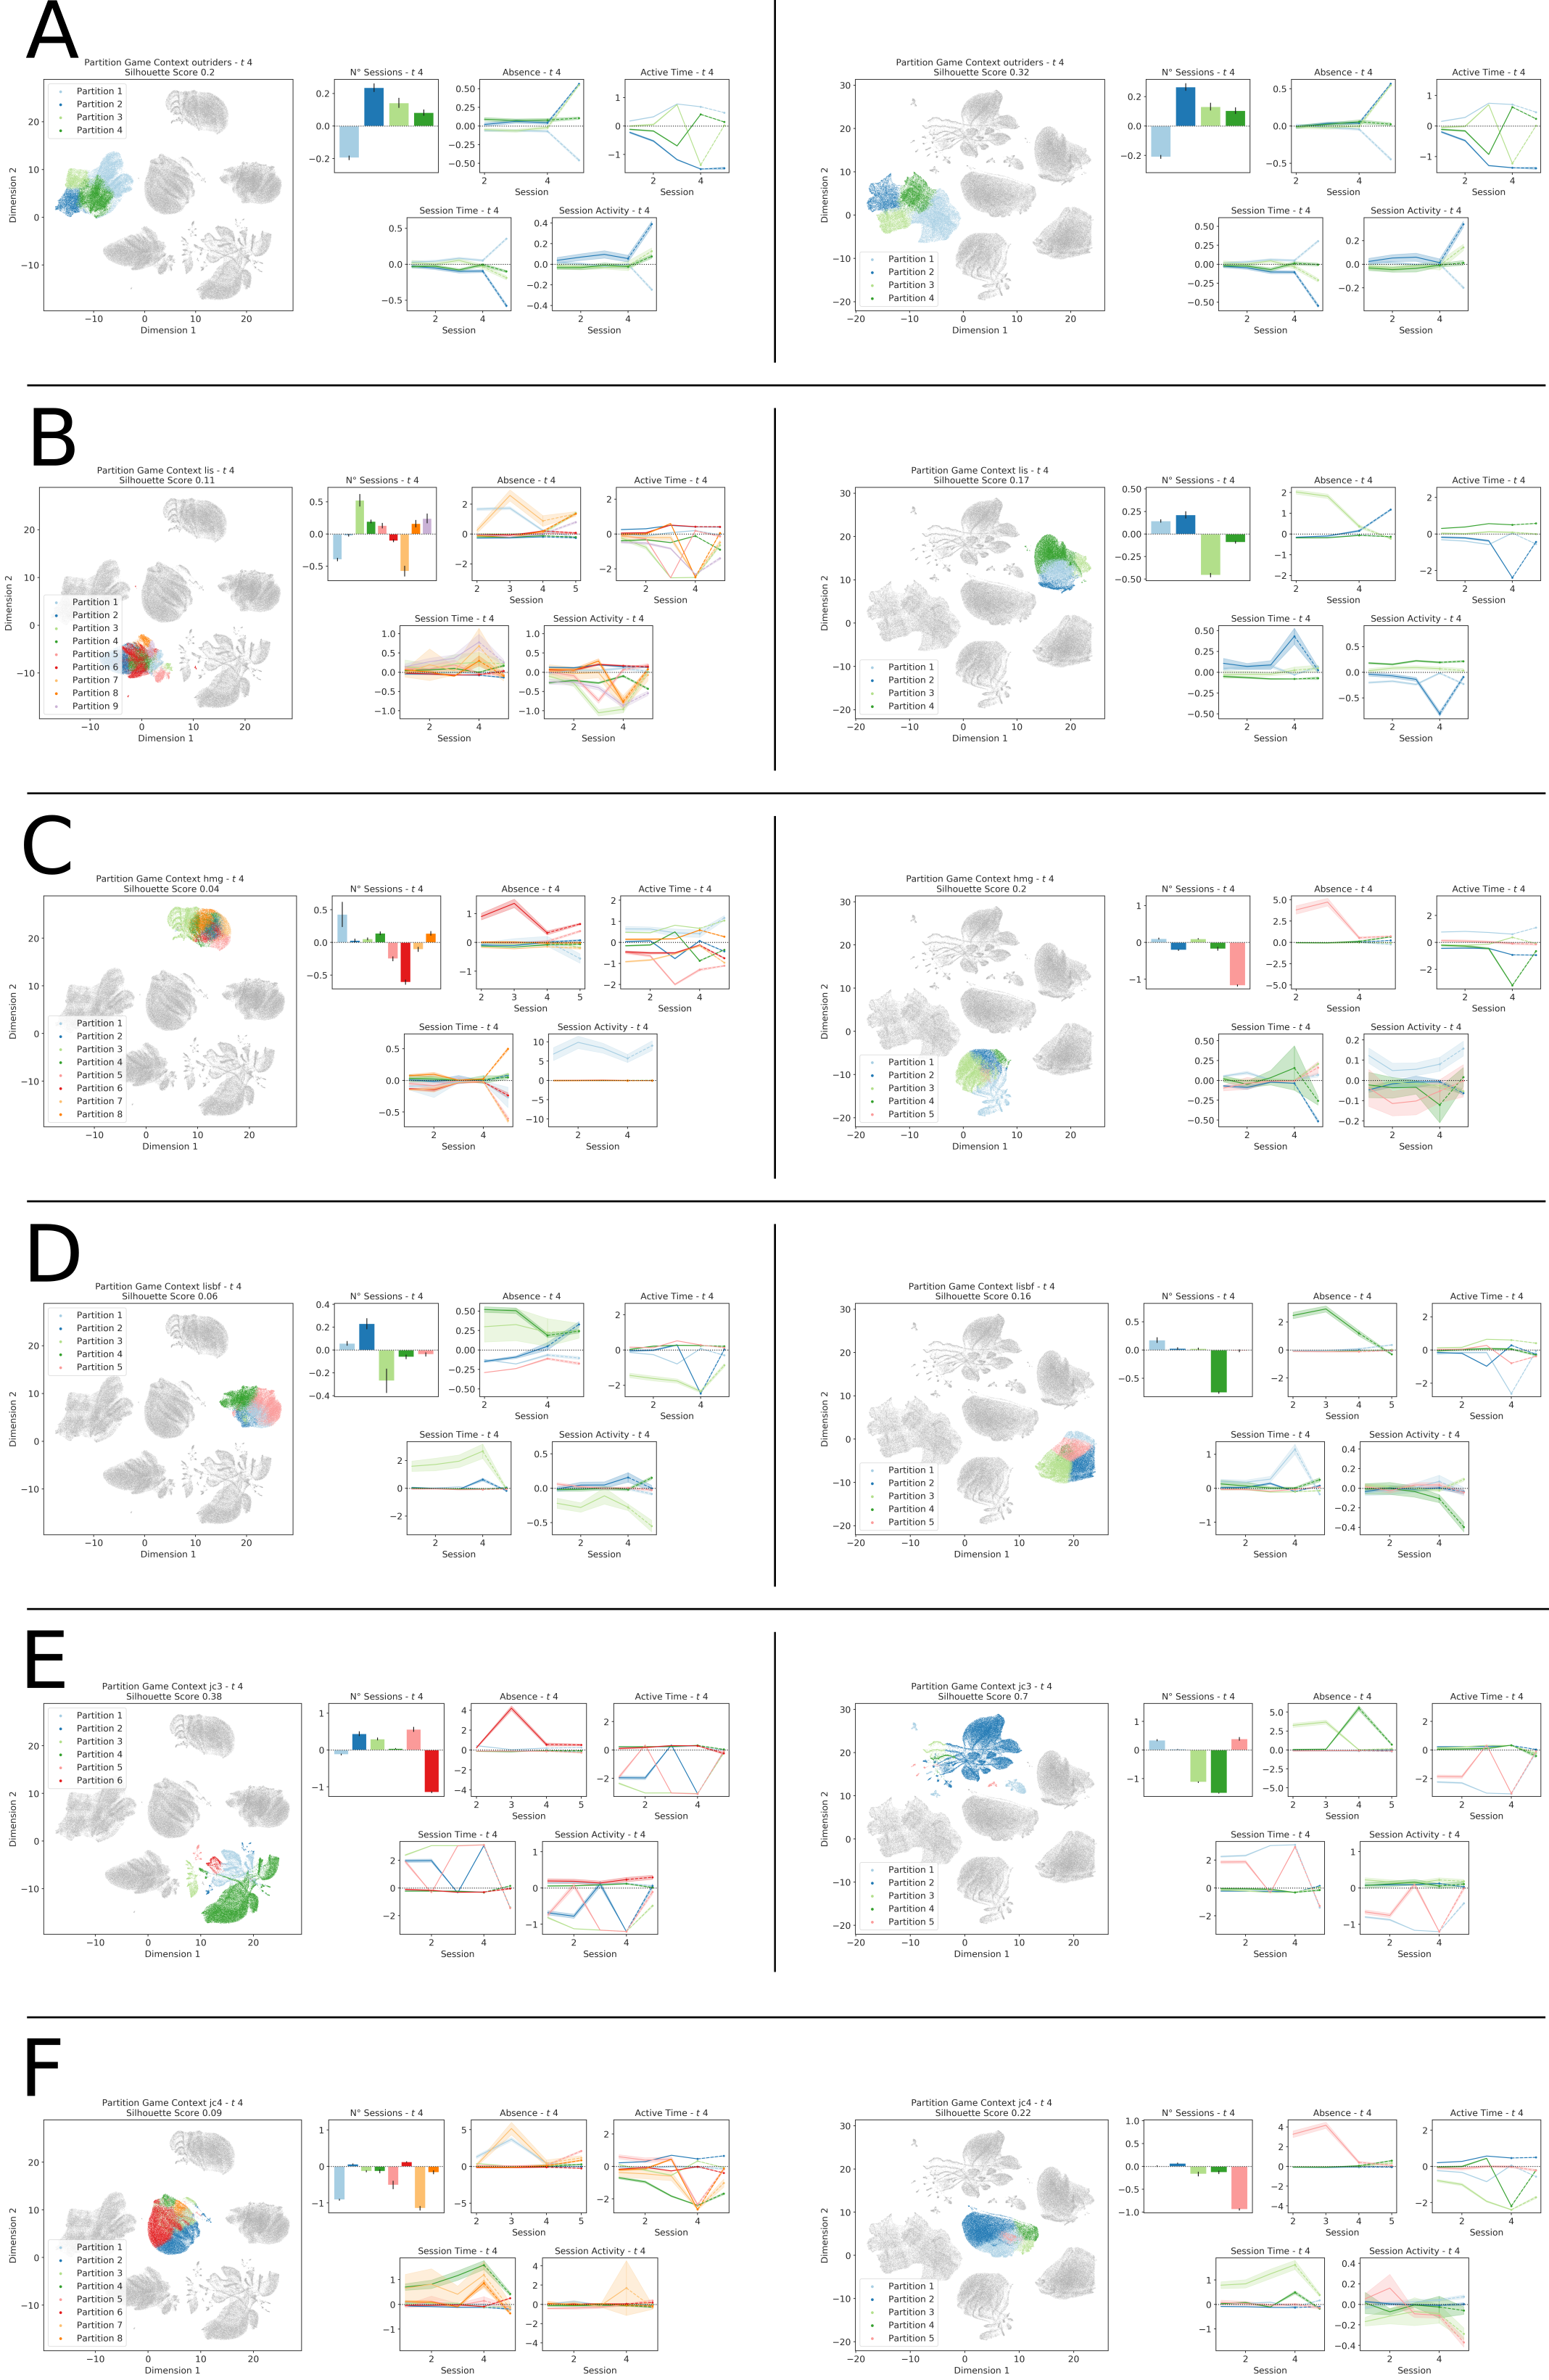
\includegraphics[width=0.8\textwidth]{images/appendix_D/clust_beha_all.png}
\centering
\caption[Partitions of the representations generated by the RNN architectures from the behavioural metrics]{The two panels show the individuated partitions and associated behavioural profiles at $t4$. The big panels report the same UMAP reduction presented in the last column of Figure \ref{full_panel_temporal}. Each dot is the representation associated with a particular individual and is colour coded based on the partition to which it belongs. Small panels represent the temporal evolution of the considered behavioural metrics for each individuated partition. The panel relative to N°Sessions only reports the prediction produced by the model as the number of preceding session is constant for all the partitions. The x axis reports the game sessions while the y axis the value assumed by the considered metric at a specific point in time. The y axis is expressed in terms of number of standard deviations from the game population mean (i.e. z-scores). Each line indicates the mean z-score while the shaded area around the line its 95\% confidence interval. The solid part of each line indicates the portion of the temporal series observed by the model (i.e. the input) while the dotted part the predictions produced at that point in time. The first columns shows the partitions associated with the representation extracted by the RNN architecture while the second those associated with the representation extracted by the version of the RNN architecture that included environmental and game events covariates. Each row reports the partitions individuated for the 6 considered game contexts.}
\label{partition_rnn_behaviour} 
\end{figure}
\FloatBarrier

\section{Partitions environmental metrics representations}
\label{partitions_environmental}

\begin{figure}[ht]
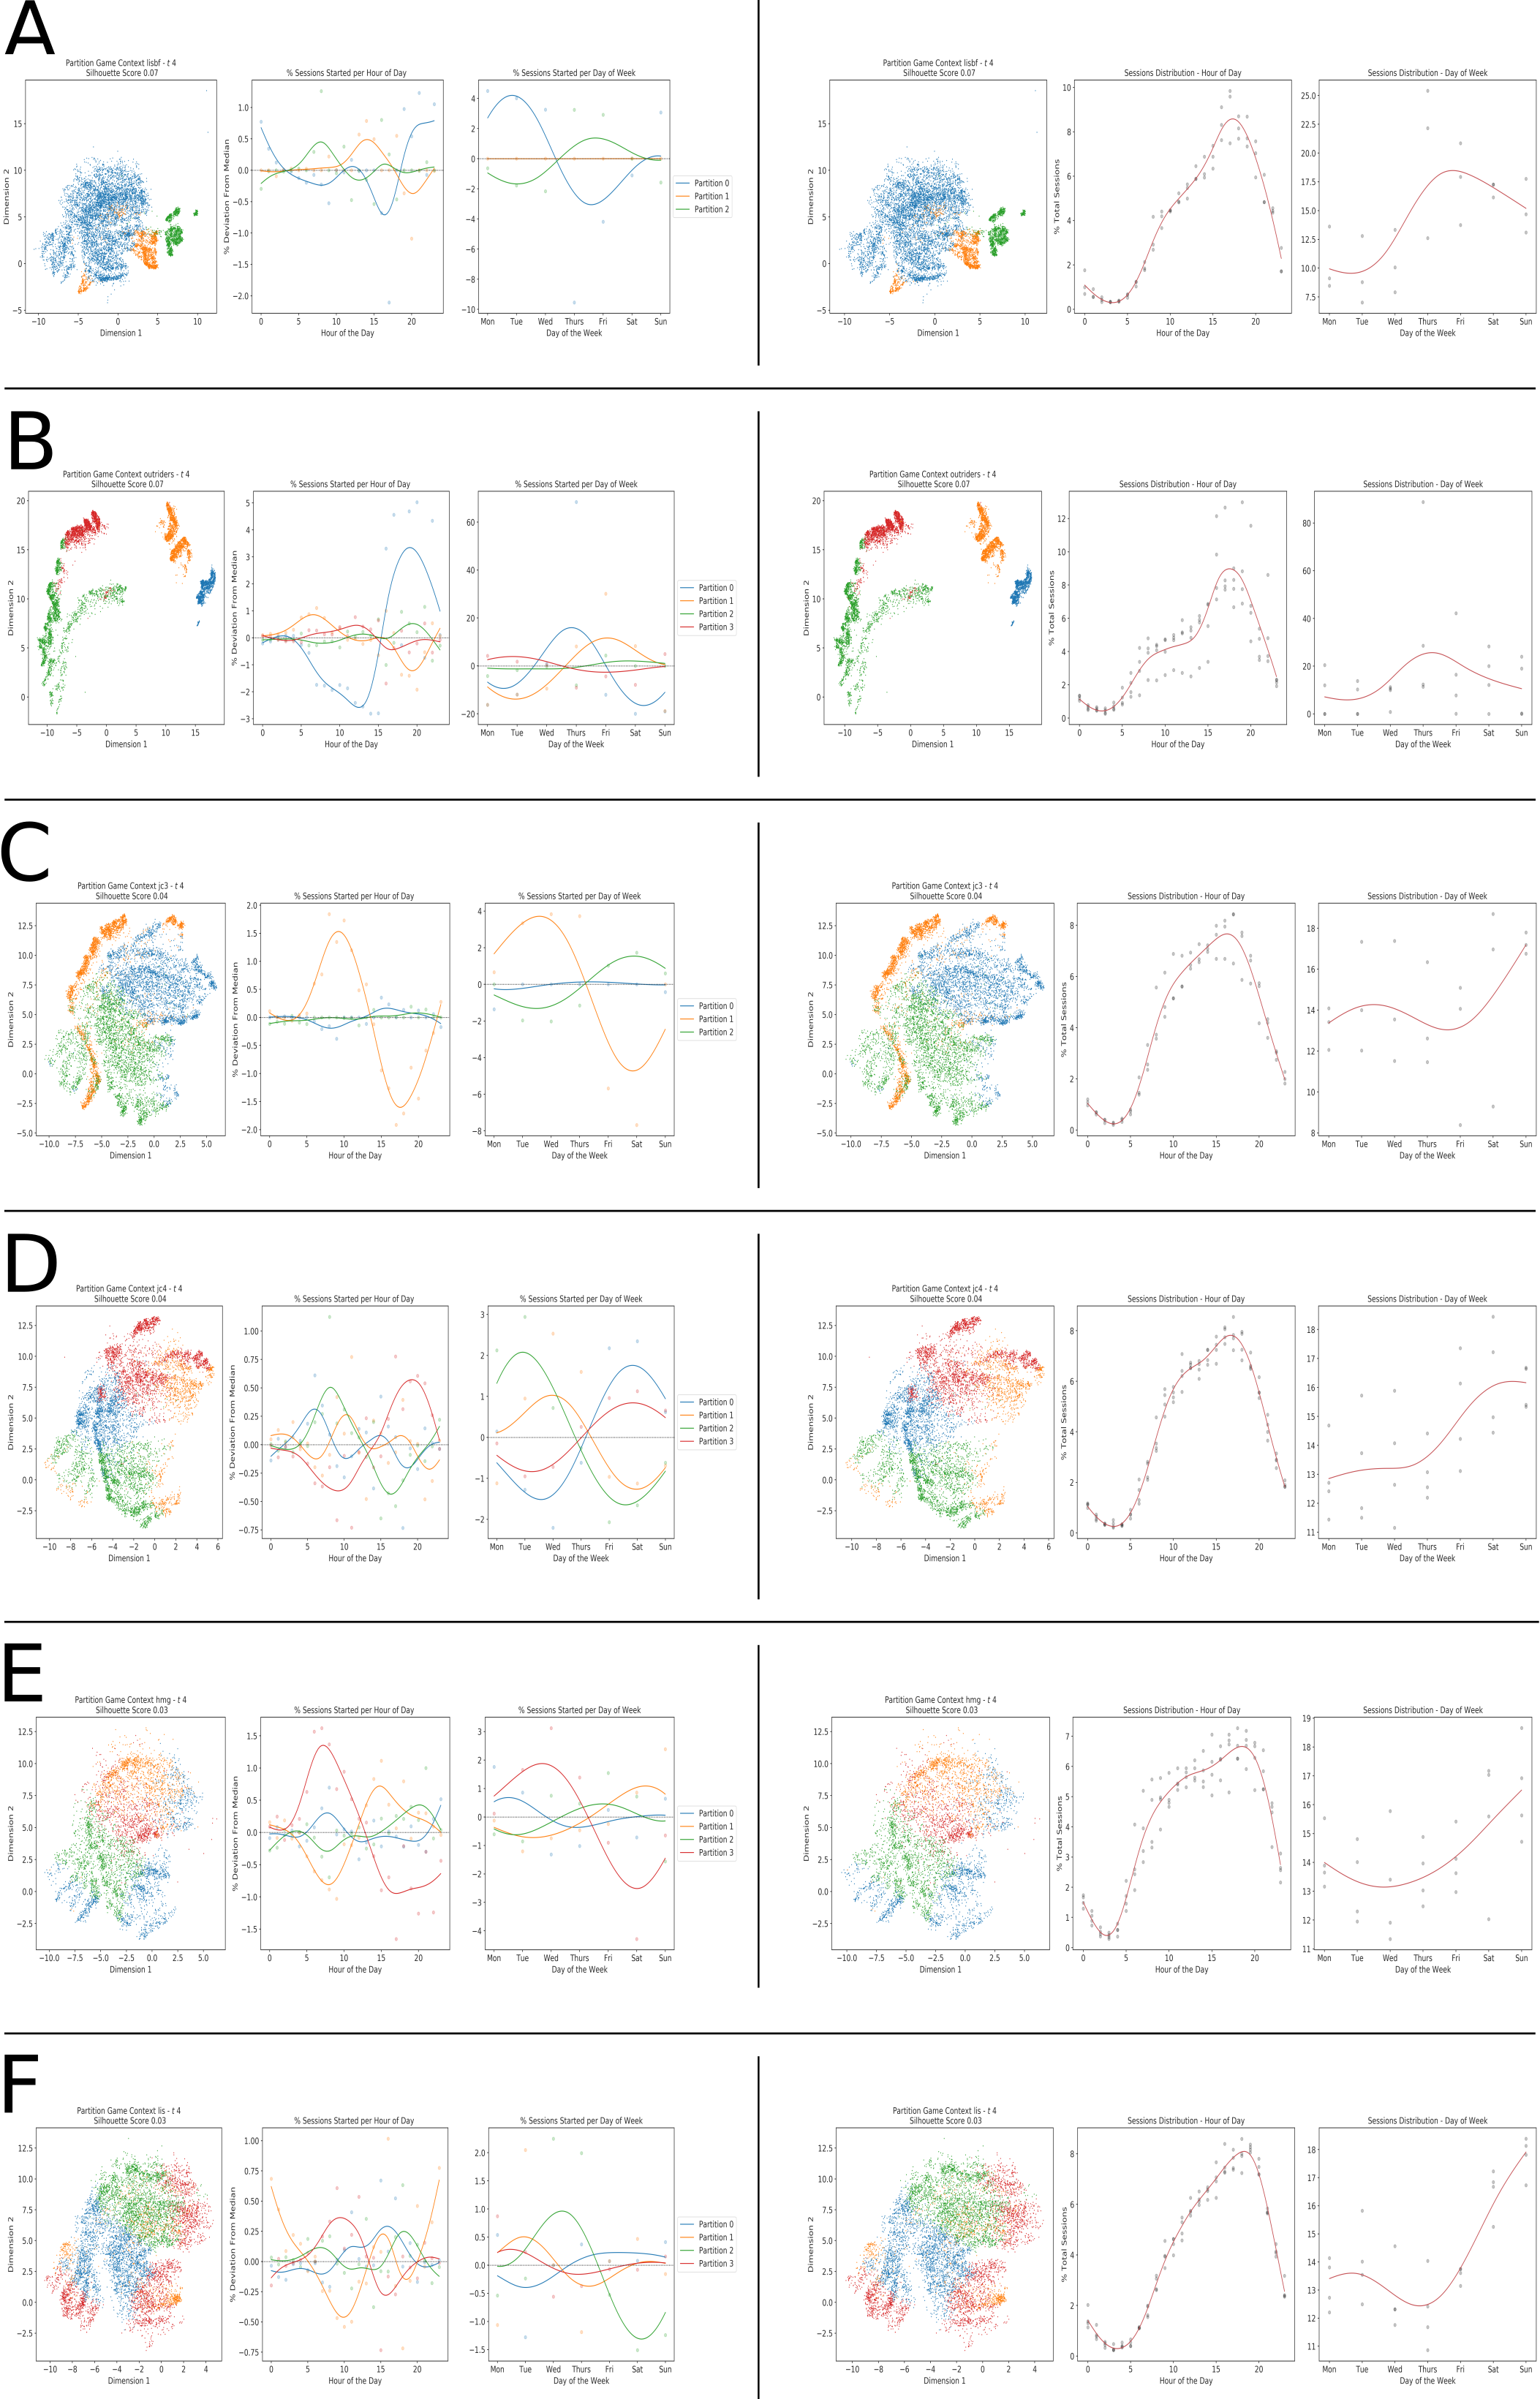
\includegraphics[width=0.8\textwidth]{images/appendix_D/clust_env_all.png}
\centering
\caption[Partitions of the representations generated by the RNN architectures from the environmental metrics]{The panels in the first row show the individuated partitions and associated profiles for the representation encapsulating all the environmental information up to $t4$. The first panel in each figure report the conventional UMAP reduction of the inferred latent representation with the colours representing the membership to a specific partition. The other two panels represent the percentage of total sessions that each partition initiated during a specific hour of the day or day of the week. The x axis reports either the hour of the day or the day of the week depending on the panel while the y axis the share of sessions expressed in terms of percentage deviations from the sample median. For each panel we reported the line of best fit provided by a generalized additive model \cite{serven2018}. The first column shows how each partition distributes its game sessions between different parts of the days or days of the week while the second column provides the same information integrated over all partitions, providing information at the sample level. Each row reports the partitions individuated for the 6 considered game contexts.}
\label{partition_rnn_env} 
\end{figure}
\FloatBarrier

\section{Partitions game events metrics representations}
\label{partitions_game_events}